\chapter{Message Passing Systems}
\label{chap:msg}

Message passing systems are probably the most common platforms for
parallel processing today.

\section{Overview}

Traditionally, shared-memory hardware has been extremely expensive, with
a typical system costing hundreds of thousands of dollars.  Accordingly,
the main users were for very large corporations or government agencies,
with the machines being used for heavy-duty server applications, such as
for large databases and World Wide Web sites. The conventional wisdom is
that these applications require the efficiency that good shared-memory
hardware can provide. 

But the huge expense of shared-memory machines led to a quest for
high-performance message-passing alternatives, first in hypercubes and
then in networks of workstations (NOWs).

The situation changed radically around 2005, when ``shared-memory
hardware for the masses'' became available in dual-core commodity PCs.
Chips of higher core multiplicity are commercially available, with a
decline of price being inevitable.  Ordinary users will soon be able to
afford shared-memory machines featuring dozens of processors.

Yet the message-passing paradigm continues to thrive.  Many people
believe it is more amenable to writing really fast code, and the the
advent of {\bf cloud computing} has given message-passing a big boost.
In addition, many of the world's very fastest systems (see
\url{www.top500.org} for the latest list) are in fact of the
message-passing type.

In this chapter, we take a closer look at this approach to parallel
processing.

\section{A Historical Example:  Hypercubes}

A popular class of parallel machines in the 1980s and early 90s was that
of \textbf{hypercubes}.  Intel sold them, for example, as did a
subsidiary of Oracle, nCube.  A hypercube would consist of some number
of ordinary Intel processors, with each processor having some memory and
serial I/O hardward for connection to its ``neighbor'' processors.

Hypercubes proved to be too expensive for the type of performance they
could achieve, and the market was small anyway.  Thus they are not
common today, but they are still important, both for historical reasons
(in the computer field, old techniques are often recycled decades
later), and because the algorithms developed for them have become quite
popular for use on general machines.  In this section we will discuss
architecture, algorithms and software for such machines.

\subsection{Definitions}

A \textbf{hypercube} of dimension d consists of \( D=2^{d} \)
\textbf{processing elements} (PEs), i.e. processor-memory pairs, with
fast serial I/O connections between neighboring PEs.  We
refer to such a cube as a \textbf{d-cube}.

The PEs in a d-cube will have numbers 0 through D-1. Let \(
(c_{d-1},...,c_{0}) \) be the base-2 representation of a PE's number.
The PE has fast point-to-point links to d other PEs, which we will call
its \textbf{neighbors}. Its i$th$ neighbor has number \(
(c_{d-1},...,1-c_{i-1},...,c_{0}) \).\footnote{Note that we number the
digits from right to left, with the rightmost digit being digit 0.}

For example, consider a hypercube having D = 16, i.e. d = 4. The PE
numbered 1011, for instance, would have four neighbors, 0011, 1111, 1001
and 1010. 

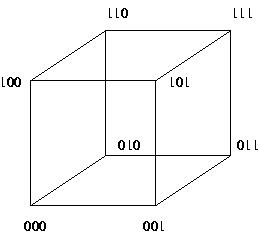
\includegraphics{Images/8cube.jpg} 

It is sometimes helpful to build up a cube from the lower-dimensional
cases.  To build a (d+1)-dimensional cube from two d-dimensional cubes,
just follow this recipe:

\begin{itemize}

\item [(a)] Take a d-dimensional cube and duplicate it. Call these two
cubes subcube 0 and subcube 1. 

\item [(b)] For each pair of same-numbered PEs in the two subcubes, add a
binary digit 0 to the front of the number for the PE in subcube 0, and
add a 1 in the case of subcube 1. Add a link between them. 

\end{itemize}

The following figure shows how a 4-cube can be constructed in this way from
two 3-cubes:

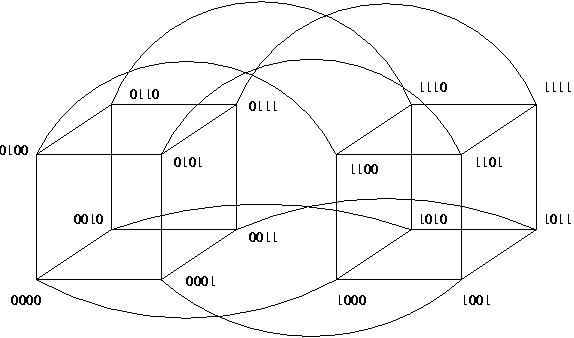
\includegraphics{Images/16cube.jpg} 

Given a PE of number \( (c_{d-1},...,c_{0}) \) in a d-cube, we will
discuss the i-cube to which this PE belongs, meaning all PEs whose first
d-i digits match this PE's.\footnote{Note that this is indeed an
i-dimensional cube, because the last i digits are free to vary.} Of all
these PEs, the one whose last i digits are all 0s is called the
\textbf{root} of this i-cube.

For the 4-cube and PE 1011 mentioned above, for instance, the 2-cube to
which that PE belongs consists of 1000, 1001, 1010 and 1011---i.e. all
PEs whose first two digits are 10---and the root is 1000.

Given a PE, we can split the i-cube to which it belongs into two
(i-1)-subcubes, one consisting of those PEs whose digit i-1 is 0 (to be
called subcube 0), and the other consisting of those PEs whose digit i-1
is 1 (to be called subcube 1).  Each given PE in subcube 0 has as its
\textbf{partner} the PE in subcube 1 whose digits match those of the
given PE, except for digit i-1.

To illustrate this, again consider the 4-cube and the PE 1011. As an
example, let us look at how the 3-cube it belongs to will split into two
2-cubes. The 3-cube to which 1011 belongs consists of 1000, 1001, 1010,
1011, 1100, 1101, 1110 and 1111. This 3-cube can be split into two
2-cubes, one being 1000, 1001, 1010 and 1011, and the other being 1100,
1101, 1110 and 1111. Then PE 1000 is partners with PE 1100, PE 1001 is
partners with PE 1101, and so on.

Each link between two PEs is a dedicated connection, much preferable to
the shared link we have when we run, say, MPI, on a collection of
workstations on an Ethernet. On the other hand, if one PE needs to
communicate with a \underbar{non}-neighbor PE, multiple links (as many
as d of them) will need to be traversed. Thus the nature of the
communications costs here is much different than for a network of
workstations, and this must be borne in mind when developing programs.

\section{Networks of Workstations (NOWs)}

The idea here is simple:  Take a bunch of commodity PCs and network them
for use as parallel processing systems. They are of course individual
machines, capable of the usual uniprocessor, nonparallel applications,
but by networking them together and using message-passing software
environments such as MPI, we can form very powerful parallel systems.

The networking does result in a significant loss of performance, but the
price/performance ratio in NOW can be much superior in many applications
to that of shared-memory or hypercube hardware of comparable number of
CPUs.

\subsection{The Network Is Literally the Weakest Link}

Still, one factor which can be key to the success of a NOW is to use a
fast network, both in terms of hardware and network protocol.  Ordinary
Ethernet and TCP/IP are fine for the applications envisioned by the
original designers of the Internet, e.g. e-mail and file transfer, but
they are slow in the NOW context.  

A popular network for a NOW today is Infiniband (IB)
(\url{www.infinibandta.org}).  It features low latency, about 1.0-3.0
microseconds, high bandwidth, about 1.0-2.0 gigaBytes per second), and
uses a low amount of the CPU's cycles, around 5-10\%.  

The basic building block of IB is a switch, with many inputs and
outputs, similar in concept to $\Omega$-net.  You can build arbitrarily
large and complex topologies from these switches.

A central point is that IB, as with other high-performance networks
designed for NOWs, uses RDMA (Remote Direct Memory Access) read/write,
which eliminates the extra copying of data between the application
program's address space to that of the operating system.

IB has high performance and scalable\footnote{The term {\it
scalable} arises frequently in conversations on parallel processing.  It
means that this particular method of dealing with some aspect of
parallel processing continues to work well as the system size increases.
We say that the method {\it scales}.} implementations of distributed
locks, semaphores, collective communication operations.  An atomic
operation takes about 3-5 microseconds.

IB implements true {\bf multicast}, i.e. the simultaneous sending of
messages to many nodes.  Note carefully that even though MPI has its
{\bf MPI\_Bcast()} function, it will send things out one at a time
unless your network hardware is capable of multicast, and the MPI
implementation you use is configured specifically for that hardware.

For information on network protocols, e.g. for example
\url{www.rdmaconsortium.org}.  A research paper evaluating a tuned
implementation of MPI on IB is available at
\url{nowlab.cse.ohio-state.edu/publications/journal-papers/2004/liuj-ijpp04.pdf}.

\subsection{Other Issues}

Increasingly today, the workstations themselves are multiprocessor
machines, so a NOW really is a hybrid arrangement.  They can be
programmed either purely in a message-passing manner---e.g. running
eight MPI processes on four dual-core machines---or in a mixed way, with
a shared-memory approach being used within a workstation but
message-passing used between them.

NOWs have become so popular that there are now ``recipes'' on how to
build them for the specific purpose of parallel processing.  The term
{\bf Beowulf} come to mean a NOW, usually with a fast network connecting
them, used for parallel processing.  The term {\it NOW} itself is no
longer in use, replaced by {\it cluster}.  Software packages such as
ROCKS (\url{http://www.rocksclusters.org/wordpress/}) have been
developed to make it easy to set up and administer such systems.

\section{Scatter/Gather Operations}
\label{scattergather}

Writing message-passing code is a lot of work, as the programmer must
explicitly arrange for transfer of data.  Contrast that, for instance,
to shared-memory machines, in which cache coherency transactions will
cause data transfers, but which are not arranged by the programmer and
not even seen by him/her.

In order to make coding on message-passing machines easier, higher-level
systems have been devised.  These basically operate in the {\bf
scatter/gather} paradigm, in which a ``manager'' node sends out chunks
of work to the other nodes, serving as ``workers,'' and then collects
and assembles the results sent back the workers.

MPI includes scatter/gather operations in its wide offering of
functions, and they are used in many MPI applications.  R's {\bf snow}
package, which will be discussed in Section \ref{snow}, is based
entirely on scatter/gather, as is MapReduce, to be discussed below.

